\section{Web Layout Background}

Complex
  web (Facebook, Amazon, GMail),
  desktop (VS Code, Figma, Slack),
  and mobile (WeChat) applications
  are driven by the interaction of two software components:
  the application itself and the browser.
The application code, typically in JavaScript,
  implements the actual application logic and
  interacts with the browser by making DOM API calls
  that modify the browser's internal representation
  of the HTML and CSS that defines the web page.
The browser code then executes its ``rendering pipeline''---%
  event handling, hit testing, matching, styling,
  layout, paint, layerizing, rastering, and drawing---%
  which reads this internal representation and transforms it,
  step by step, into pixels on the screen.
Application code is typically most of the execution time
  but that code's effects are ultimately visible to the user
  only through ``system calls'' serviced by browser-level code.
For the application to be responsive and smooth,
  those calls  have to be serviced
  in 16 milliseconds (60 frames per second).

Concretely, a browser application is written in HTML,
  which defines a tree called the ``document'',
  whose nodes include text, buttons,
  and structural elements like \texttt{div}s.
The application code binds specific callback functions
  to user actions like clicking on certain elements,%
  \footnote{Callbacks can also run in response to
    timers, network requests, or a dizzying array of
    other events.}
  and these callbacks can modify the HTML using DOM methods
  like \texttt{appendChild} or \texttt{setAttribute}.
When the callback finishes executing,%
\footnote{Or after multiple callbacks finish executing,
  as decided by the browser's task scheduler.}
  the browser executes the full rendering pipeline
  to display the results to the user.
Some DOM methods like
  \texttt{getBoundingRect} or \texttt{offsetX}
  read state computed during the rendering pipeline;
  calling these methods can requires the browser
  to perform additional passes through the rendering pipeline,
  and is necessary for common interactions like tooltips.

\subsection{The Layout Phase}

\begin{figure}[tbp]
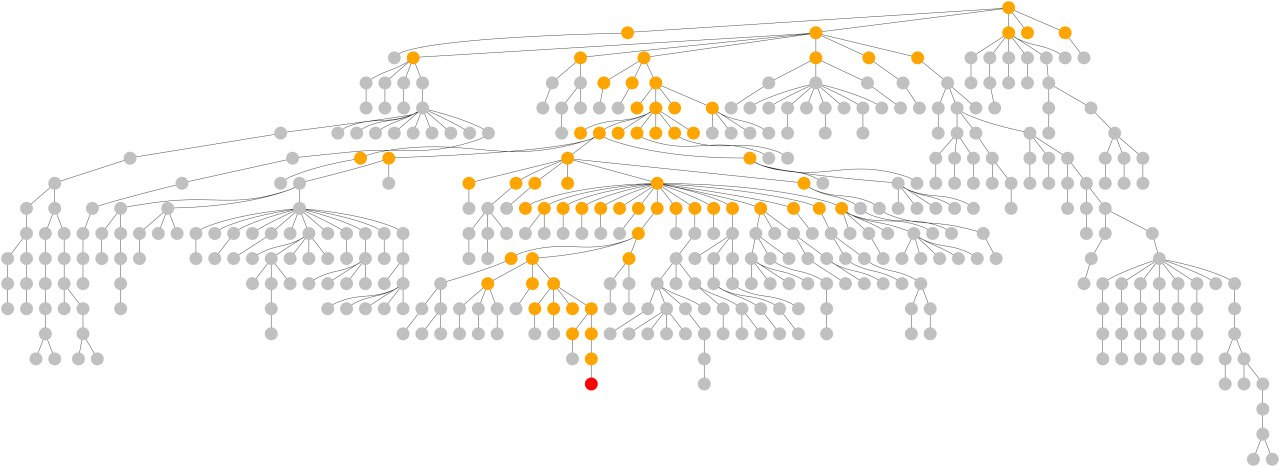
\includegraphics[scale=0.3]{tree.jpg}
\caption{The DOM tree for \texttt{google.com}, with 842 total nodes, a maximum fanout of 16, and a maximum depth of 18. The node marked red is part of the auto-complete suggestion box. The node color corresponds to the Double Dirty Bit algorithm, with gold representing auxiliary nodes and gray representing skipped nodes. Auxiliary nodes are a large fraction of the page even when only one node is (transitively) dirtied.
}
\label{fig:google}
\end{figure}

This paper is specifically concerned with the layout phase,
  a long-term focus of the programming languages community.
The layout phase traverses an intermediate structure
  called the ``layout tree'' and computes, for each node,
  a set of ``layout fields''
  including each element's size and position.
This computation proceeds in several passes,
  first computing intermediate layout fields
  like intrinsic width and height
  and current line ascent/descent
  before computing size and position.

The layout tree is basically the HTML tree,
  with minor differences like
  ``generated content'' (like bullets for list items)
  and ``fragmentation'' (like line breaking)
  that are not critical to this paper.
The trees are both big and unbalanced;
  the famously minimal Google home page page, for example,
  has 842 nodes, with a maximum fanout of 16 and depth of 18;
  it is drawn in \Cref{fig:google}.
In memory, the layout tree is stored as a pointer tree,
  with the children of each node stored in a doubly-linked list.%
\footnote{
This ensures that node insertions and deletions are fast,
  even in poorly-balanced trees.
}
The application can add or remove nodes from this tree,
  or write to their ``properties'' and ``attributes'',
  to update what the user sees.

Each node's layout fields depend on the layout fields
  of its neighbors.
For example, imagine a paragraph containing several lines;
  both the paragraph and each line would correspond
  to a layout node.
The height of the paragraph, in this case,
  would be the sum of the heights of all its children
  plus any gaps between them,
  while a node's width would be its parent's width,
  minus some padding.
Of course, real-world web layout is much more complex;
  Chrome's implementation is about 100,000 lines of code
  and computes hundreds of fields per node.
To compute all these fields correctly, the layout algorithm
  recursively traverses the tree multiple times.
For example, the layout algorithm might first compute
  the intrinsic size of each element in a bottom-up traversal;
  then compute preferred sizes, in a top-down traversal;
  and then apply flexible sizing rules in a bottom-up traversal
  to finally compute each element's actual size.
Note that not only are multiple passes necessary,
  but that each pass must visit the nodes of the layout tree
  in a specific order so that each layout field's dependencies
  are satisfied.

\begin{figure}
    \centering
    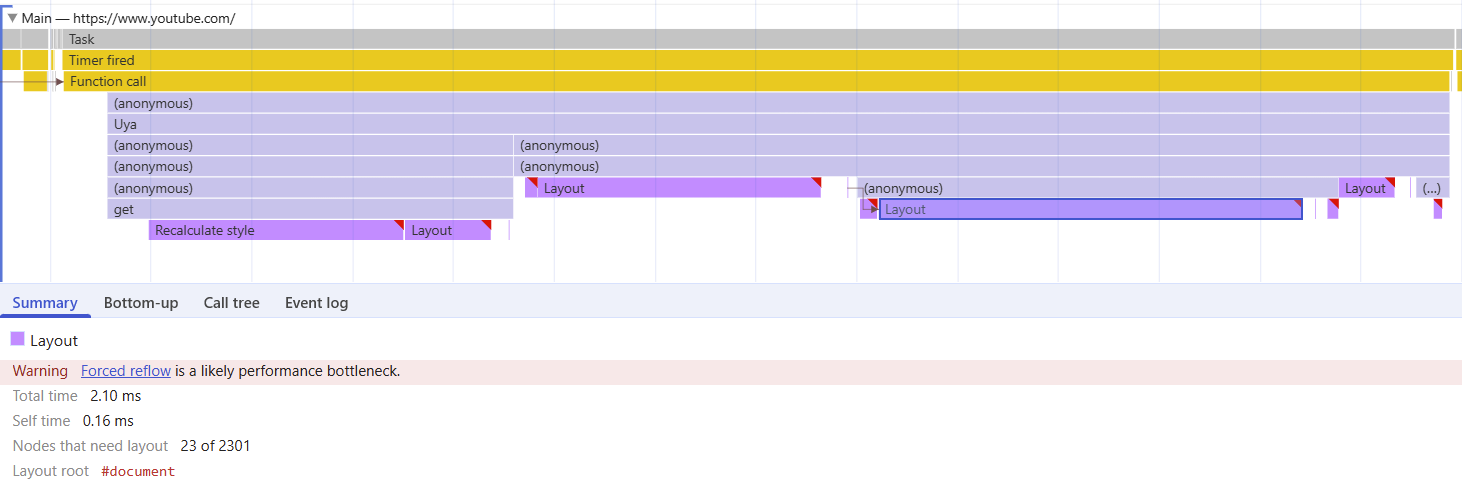
\includegraphics[width=\linewidth]{profile.png}
    \caption{
      A trace of nine milliseconds of Chrome opening Youtube;
        time flows left to right while the call stack grows down.
      The violet ``recalculate style'' and ``layout'' blocks
        are phases of the browser rendering pipeline,
        with layout in total consuming four milliseconds;
        the faint vertical lines are half-millisecond marks.
      Layout happens multiple times in one frame
        due to ``forced reflows''.
      The ``Summary'' tab at the bottom shows
        that the selected (longest) layout
        only updates 23 of 2\thinspace01~nodes
        in the layout tree.}
    \label{fig:profile}
\end{figure}

\Cref{fig:profile} shows layout performance in practice:
  a trace of Google Chrome opening YouTube,
  captured and visualized using Chrome's ``Performance'' tools.
The trace covers 9~milliseconds of execution time,
  with time running left to right.
Function calls grow downward, and the leaves,
  labeled ``recalculate style'', ``layout'',
  and ``pre-paint'' (barely visible)
  are different phases of the rendering pipeline;
  the application-level code is offscreen to the left.
In these nine milliseconds,
  the application requests layout four times
  due to calling APIs that require (``forced reflow'')
  multiple passes through the rendering pipeline.
These four layout each take more time than
  the browser developers' target latency,
  as indicated by the red tags on these blocks.

Below the trace, the ``Summary'' tab shows
  more information about a single, selected layout
  taking 2.1~milliseconds.
This layout operated
  on a layout tree of 2\thinspace301~nodes,
  starting from the root of the web page (\texttt{\#document}).
However, it only needed to update 23~of~them;
  in other words, this layout was incremental.
The long running time of the layout phase
  nonetheless caused unacceptable latency;
  in fact, this frame ``drops'',
  meaning the browser isn't able to update the page
  in time to show smooth animations and interactions.

\subsection{Formal Modeling}

Luckily, the programming languages community
  has developed a sophisticated understanding of layout.
Early work by Meyerovich and others%
  ~\cite{meyerovich-1,meyerovich-2,meyerovich-3}
  developed ``attribute grammars'' as a formalism
  for defining layout rules and implementations.
The later Cassius project~\cite{cassius-1,cassius-2,cassius-3}
  developed a full, standards-compliant implementation
  of a significant fragment of the layout rules
  in this formalism,
  and the \textsc{Hecate} and \textsc{Medea}
  tools~\cite{yufeng-1,yufeng-2}
  have shown that automatic synthesis can be scaled
  to such fragments.  

\begin{figure}
\begin{align*}
\text{Layout} &\coloneq  \text{Rule}^+; \textbf{schedule}\:\text{Pass}_n^+ \\
\text{Rule} &\coloneq
  \mathbf{def}\:\text{Pass}_n()\:\{\:
    A^+;\:
    \mathsf{children}.\mathsf{forEach}(\text{Pass}_n);\:
    A^+;\:
  \} \\
A \in \text{Assignment} &\coloneq
  \text{self}.V \leftarrow T \\[4pt]
T \in \text{Term} &\coloneq
  \text{if}\ T\ \text{then}\ T\ \text{else}\ T \mid
  F(T^+) \mid
  N? \mid
  N.V \mid
  \mathsf{attribute}[V] \mid
  \mathsf{property}[V] \\
N \in \text{Neighbor} &\coloneq
  \mathsf{self} \mid \mathsf{prev} \mid
  \mathsf{next} \mid \mathsf{parent} \mid
  \mathsf{first} \mid \mathsf{last} \\[4pt]
V \in \text{Variable} &\coloneq \text{layout fields} \quad\quad
F \in \text{Function} \coloneq \text{primitive functions}
\end{align*}
\caption{
  A minimal DSL for defining web layout
    as a set (\textsf{rules}) of passes
    performed in a specific order (\textsf{schedule}).
  The syntax $P^+$ represents a sequence of non-terminal $P$.
  Passes are in-order traversals of the layout tree
    performing a sequence of assignments to local fields
    while accessing fields of the current node or its neighbors.
}
\label{fig:dsl}
\end{figure}

\Cref{fig:dsl} defines an attribute grammar.
In an attribute grammar, a layout is defined by
  a set of passes (the rules)
  performed in a certain order (the schedule).
Each pass performs a recursive, in-order traversal of the tree,
  computing some fields pre-order and some fields post-order;
  every field is written to exactly once in exactly one pass.
For each field assignment $\mathsf{self}.V \gets T$,
  the expression $T$ can refer
  to fields of $\mathsf{self}$ or
  to fields of its $\mathsf{parent}$,
  $\mathsf{prev}$ and $\mathsf{next}$ sibling,
  or $\mathsf{first}$ and $\mathsf{last}$ child;
  expressions can also test whether a given neighbor
  exists ($\mathsf{N?}$).
Computations can also refer to
  attributes or properties of the current node
  using $\mathsf{attribute}[x]$ or $\mathsf{property}[x]$.%
\footnote{
The split HTML attributes and CSS properties
  use two different namespaces
  because some names, like \texttt{height},
  appear in both sets.
There is no other semantic difference between them,
  and other accessible properties,
  such as the tag name or image width and height
  are modeled in our system as special properties.
}
All computations besides field assignments are pure,
  there are no other loops or data structures,
  and the only field access allowed is to a node's neighbors.
Despite this, even complex layout features
  like flexible box layout are expressible in such a DSL.

\begin{figure}
\begin{minipage}[b]{0.68\linewidth}
\begin{align*}
& \mathbf{def}\:\text{Pass}_1()\:\{ \\
& \quad \mathsf{self}.W \gets
        \mathbf{if}\:\mathsf{parent}?\:
        \mathbf{then}\:\operatorname{max}(0, \mathsf{parent}.W - 10)\:
        \mathbf{else}\:50; \\
& \quad \mathsf{children}.\mathsf{forEach}(\text{Pass}_1); \\
& \quad \mathsf{self}.H \gets
        \mathbf{if}\:\mathsf{last}?\:
        \mathbf{then}\:\mathsf{last}.HA + 10\:
        \mathbf{else}\:\mathsf{self}.\text{attribute}[\mathsf{height}]; \\
& \quad \mathsf{self}.HA \gets
        \mathbf{if}\:\mathsf{prev}?\:
        \mathbf{then}\:\mathsf{prev}.HA + \mathsf{self}.H + 5\:
        \mathbf{else}\:\mathsf{self}.H; \\
& \} \\
& \mathbf{schedule}\:\text{Pass}_1
\end{align*}
\caption{
  A minimal paragraph layout implementation,
    computing width $W$ and height $H$,
    with 5 pixels padding and 5 pixel gaps between lines.
  The intermediate $HA$ field sums the height
    of a node and all its previous siblings and gaps.
  This simple layout algorithm has one pass,
    but real-world layouts contain multiple.
}
\label{fig:layout-simple}
\end{minipage}\hfill%
\begin{minipage}[b]{0.28\linewidth}
\centering
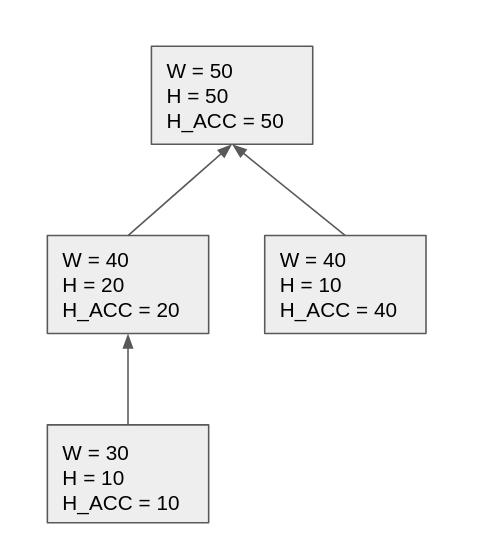
\includegraphics[scale=0.23]{LayoutExample.png}
\caption{The layout algorithm running on a layout tree of size 4. All nodes have an height attribute of 10.
}
\end{minipage}
\end{figure}
\Cref{fig:layout-simple} shows
  the layout example for paragraphs and lines,
  defined using an attribute grammar.
Here the nodes are the paragraphs and lines,
  and they all have three layout fields:
  a width $W$, a height $H$, and an intermediate field $HA$
  that computes the height of a node and its previous siblings
  (plus any gaps between lines).
Width information propagates from parents to children,
  starting at 50 pixels and subtracting, at each level,
  5 pixels of padding on the left and right.
Height information propagates from children to parents---%
  a node's height is the sum of its children's heights,
  plus 5-pixel gaps between lines---%
  and relies on the intermediate $HA$ field
  which propagates information from previous to next siblings.
Note that the idea of ``summing all children's heights''
  is not expressed with a loop;
  instead, it is expressed as an additional layout field,
  which has its own computation rule.

Attribute grammar DSLs can be heavily optimized.
The layout fields can stored in the node itself,
  tightly packed to ensure locality.
Computations can use primitive data types
  like integers, floats, and enumerations;
  strings can be interned and hash tables statically flattened.
The only pointer accesses are to neighboring nodes,
  which are likely to be in cache.
Branch mis-prediction are relatively rare
  given the minimal control flow.
The tree structure itself does not change \emph{during layout}.
This efficiency is critical to browser developers.

A key property of attribute grammar DSLs like this one
  is that dependencies and traversal orders are static.
Specifically, for any field assignment,
  examining the expression $T$ reveals
  which other fields on which other nodes it depends on.
These static dependencies are critical for invalidation.
Also, the schedule language ensures that
  the relative order in which two fields are computed
  never changes, even as nodes are added or removed.
This is critical for Spineless Traversal.
In this paper, we assume that this schedule
  respects the field dependencies
  and that the rules have no cyclic dependencies;
  we also assume that the schedule has already been optimized
  by fusing traversals and ordering field assignments.
A substantial literature exists on these topics~%
  \cite{grafter,yufeng-1,yufeng-2},
  and the layout implementation used in our evaluation
  is detailed in Section~\ref{sec:layout-impl}.
In any case, while this paper focuses on web layout,
  we expect Spineless Traversal to be applicable
  to incremental computations in other domains,
  including in compilation, static analysis,
  computer graphics, and databases,
  as long as they can be expressed as an attribute grammar
  in this or a similar DSL.